%!TEX root = ../physical-olympics-2.tex
\chapter{弹性体}


\section{弹性体的物理描述}

所谓弹性体就是完全\emph{弹性}(elasticity)的物体.\,弹性描述的是使物体发生形变的力撤除以后物体可以回到静息状态的属性.\,弹性力学研究的对象与范围就是弹性体的力学性质.\,一般来说,\,固体主要具有弹性而液体主要具有黏性,\,若是研究中间的状态,\,\emph{非牛顿流体}(non-newtonian fluid)和\emph{塑性固体}(plastic solid),\,那就是\emph{黏弹性力学}(rheology)要研究的对象了.\,典型的黏弹性过程受力不是简单地正比于位移而是与速度,\,与历史相关.\,因此而可以发生永久的不可恢复的变形.

正因为如此,\,完整描述弹性体的运动学时,\,不得不额外留心所有点的实际位移.\,在流体时也许速度更需要注意.\,所以我们写出一个初始$t=0$位置矢量为$\bs{R}$的点,\,经过$t$时间到达位置为$\bs{r}$处,\,也就是我们要定义一个$\mathrm{3D}\times\mathrm{1D}$到$\mathrm{3D}$的映射:
\[\bs{r}=\bs{r}(\bs{R},t)\]

不失普遍性地,\,我们考虑如何刻画在$\bs{R}=\bs{0}$的形变.\,我们需要研究在$\bs{R}=\bs{0}$的附近$\ud \bs{R}=\ud X\bs{e}_x+\ud Y\bs{e}_y+\ud Z\bs{e}_z$处的位移$\bs{\delta}=\bs{r}-\bs{R}$与中心的位移去比较.\,数学上有以下泰勒展式:
\[\bs{\delta}(\ud \bs{R},t)=\bs{\delta}(\bs{0},t)+\ud \bs{R}\cdot \nabla \bs{\delta}\]

上式中$\nabla\bs{\delta}$是一个有九个分量的张量,\,张量这一概念上一章介绍过,\,它是九个分量的三行三列式的组合,\,现在它的作用是可以与之前的矢量$\ud \bs{R}$点乘把它线性地映射为另一个矢量:
\[\nabla\bs{\delta}=\sum_{i,j}\frac{\partial \delta_j}{\partial X_i}\bs{e}_i\bs{e}_j\]
\[\nabla\bs{\delta}:\; \sum_i\ud X_i\bs{e}_i\rightarrow \sum_j\ud \delta_j\bs{e}_j=\sum_j\left(\sum_i \frac{\partial \delta_j}{\partial X_i}\ud X_i\right)\bs{e}_j\]

\[\nabla\bs{\delta}:\; \begin{bmatrix}\frac{\partial \delta_x}{\partial X}&\frac{\partial \delta_y}{\partial X}&\frac{\partial \delta_z}{\partial X}\\\frac{\partial \delta_x}{\partial Y}&\frac{\partial \delta_y}{\partial Y}&\frac{\partial \delta_z}{\partial Y}\\\frac{\partial \delta_x}{\partial Z}&\frac{\partial \delta_y}{\partial Z}&\frac{\partial \delta_z}{\partial Z}\end{bmatrix}\]

不难发现第二个式子是不证自明的.\,所以实际上刻画形变的包含于$\nabla\bs{\delta}$这个张量.\,但是并不是完全取决于它,\,考虑像刚体这样的不能变形的物体,\,上一章介绍过,\,旋转依然是可能的.\,不妨设刚体不仅随$\bs{R}=\bs{0}$的点发生了$\bs{\delta}(\bs{0},t)$式的平动,\,也要发生一个$\ud\bs{\phi}$的小角度转动.\,在这里我们让转动的角度足够小以至于可以做小角近似.\,这样就可以把刚体式的位移的以上张量写成:
\[\bs{\delta}(\ud \bs{R},t)=\bs{\delta}(\bs{0},t)+\ud \bs{\phi}\times \ud \bs{R}\]
\[\nabla\bs{\delta}:\; \begin{bmatrix} 0&\ud \phi_z &-\ud \phi_y \\-\ud \phi_z&0&\ud \phi_x \\ \ud \phi_y &-\ud \phi_x &0\end{bmatrix}\]

这个矩阵是一个反对称矩阵,\,从而我们得出一个结论:\,一个固体在某点位移对应的$\nabla\bs{\delta}$如果是反对称的,\,则不产生任何形变,\,仅仅是局部整体发生了平移和旋转.

但是有一个简单的定理.\,任何一个方矩阵$[M_{ij}]$都能被唯一地分解为对称矩阵和反对称矩阵.\,分别称作原来矩阵的\emph{对称部分}(symmetric component)和\emph{反对称部分}(anti-symmetric component).\,用矩阵的转置可以很简单的得到这个结果:
\[[M_{ij}]=[S_{ij}]+[A_{ij}]\]
\[[S_{ij}]=\frac{[M_{ij}]+\phantom{}^{\rm t}[M_{ij}]}{2}\quad,\quad [A_{ij}]=\frac{[M_{ij}]-\phantom{}^{\rm t}[M_{ij}]}{2}\]

那么问题就很简单了,\,之前那个矩阵的对称部分就是描述形变的部分.\,这个部分被叫做\emph{应变张量}(strain tensor),\,以后用$\bs{\varepsilon}$来表示\footnote{本书印刷体张量都是与矢量一致的粗体.\,手写时,\,为了区分,\,可以把张量写作带异型箭头的形式$\stackrel{\leftrightarrow}{T}$或者直接用自由指标的分量代指构成的整体$T_{ij}$.}:
\[\bs{\varepsilon}=\frac{1}{2}(\nabla\bs{\delta}+\phantom{}^{\rm t}\nabla\bs{\delta})\]
\[\bs{\varepsilon}:\; \begin{bmatrix}\frac{\partial \delta_x}{\partial X}&\frac{1}{2}\frac{\partial \delta_y}{\partial X}+\frac{1}{2}\frac{\partial \delta_x}{\partial Y}&\frac{1}{2}\frac{\partial \delta_z}{\partial Y}+\frac{1}{2}\frac{\partial \delta_y}{\partial Z}\\\frac{1}{2}\frac{\partial y}{\partial X}+\frac{1}{2}\frac{\partial \delta_x}{\partial Y}&\frac{\partial \delta_y}{\partial Y}&\frac{1}{2}\frac{\partial \delta_x}{\partial Z}+\frac{1}{2}\frac{\partial \delta_z}{\partial X}\\\frac{1}{2}\frac{\partial \delta_z}{\partial Y}+\frac{1}{2}\frac{\partial \delta_y}{\partial Z}&\frac{1}{2}\frac{\partial \delta_x}{\partial Z}+\frac{1}{2}\frac{\partial \delta_z}{\partial X}&\frac{\partial \delta_z}{\partial Z}\end{bmatrix}=\begin{bmatrix} \varepsilon_x&\theta_{xy}/2 &\theta_{zx}/2 \\ \theta_{xy}/2&\varepsilon_y&\theta_{yz}/2 \\ \theta_{zx}/2&\theta_{yz}/2&\varepsilon_z\end{bmatrix}\]

\begin{wrapfigure}[15]{o}[-10pt]{7cm}
\vspace{-0.5cm}
\centering
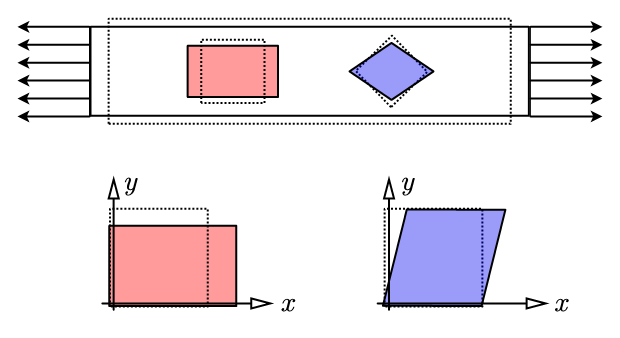
\includegraphics[width=7cm]{image/6-7-1.png}
\caption{正应变与剪应变}\label{6-7-1}
\end{wrapfigure}
其中三个对角元素$\varepsilon$称作\emph{正应变}(normal strain).\,而非对角的元素$\theta$称作\emph{剪应变}(shear strain).\,如图\ref{6-7-1}所示,\,在一种非常简单的模型中,\,大气中的棒被在沿棒方向施加一个拉力而伸长,\,但宽方向很自然地会产生些许的收缩.\,那么根据在棒里取出不同的微元形式,\,其变形方向也会有所改变.\,红色部分沿$x$方向就发生了明显的正应变.\,这是因为合适地平移,\,旋转其变形后的微元对齐形变前的微元(虚线)后,\,明显发现在$x$方向长度变大了.\,如果初始长度为$X$,\,之后在微元范围内端点的$x=X+\delta$.\,于是根据上面的定义,\,正应变其实就是:
\[\varepsilon=\frac{\delta}{X}=\frac{x-X}{X}\]

而蓝色部分是个平行四边形,\,将底边与变形前的底边对齐以后,\,我们发现$x-y$平面上顶角不再是$90^\circ$,\,这其实就标志着剪应变.\,如果这个角度减小了$\alpha$,\,那么之后的$x=X+Y\tan\alpha,\,y=Y$.\,这就说明$\delta_x=Y\tan\alpha,\,\delta_y=0$.\,从而:
\[\theta_{xy}=\frac{\partial \delta_y}{\partial X}+\frac{\partial \delta_x}{\partial Y}=\tan\alpha\approx \alpha\]

可见这个角度变化其实就是剪应变,\,它与边的对齐方式无关,\,如果$x,\,y$轴夹角变小便是正的.\,正应变,\,剪应变都是无量纲的物理量.

\vspace{0.5cm}

接下来需要考虑弹性体的内部受力情况.\,令人惊讶的是,\,它也必然由一个对称张量描述.\,首先我们意识到弹性力内部的受力具有以下特征:\,A.\,是空间点的函数,\,不同点处可以不同,\,但每一点应当有一个受力情况,\,它就是内部的\emph{应力}(stress).\,B.\,不是一个矢量.\,显然指出弹性体中的一点,\,并不能马上对应出来这个点处的某个受力的情况,\,因为我们考虑的是内力而不是外力,\,但是点处的受力不可能有明确的施力物体与受力物体.\,那么其实还需要在这一点处找到一个面矢量$\ud \bs{S}$,\,才能说是谁对谁的力.\,我们这样就发现了,\,其实指定一个应力,\,本质上就是在每一点指定一个面矢量$\ud \bs{S}$到相互作用力$\ud \bs{F}$的映射.\,C.\,显然,\,这样的映射应当为线性映射\footnote{证明留给读者做思考,\,需要用到极限微元受力分析.}.

\begin{wrapfigure}[15]{o}[-10pt]{7cm}
\vspace{-0.5cm}
\centering
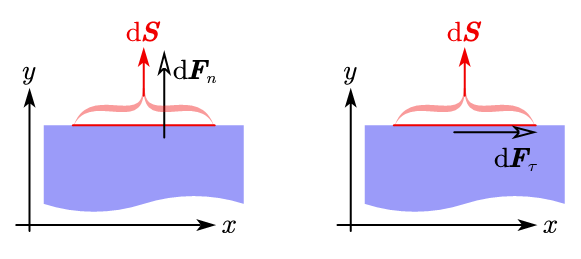
\includegraphics[width=7cm]{image/6-7-2.png}
\caption{正应力与剪应力}\label{6-7-2}
\end{wrapfigure}
这样就几乎已经说明,\,应力其实就是一个张量.\,因为从一个矢量$\ud \bs{S}$到另一个矢量$\ud \bs{F}$的线性映射的数学模型其实就是张量,\,它存在$3\times 3=9$个分量.\,我们进一步指定,\,$\ud \bs{F}$的含义$\ud \bs{S}$指向的那一侧的体元对这一侧的体元通过$\ud \bs{S}$施加的相互作用力.\,这个张量就是:
\[\left\{\begin{array}{ccc}\ud F_x &= & \sigma_{xx} \ud S_x + \sigma_{xy} \ud S_y+\sigma_{xz} \ud S_z \\ \ud F_y&= & \sigma_{yx} \ud S_x + \sigma_{yy} \ud S_y+\sigma_{yz} \ud S_z \\ \ud F_z &= & \sigma_{zx} \ud S_x + \sigma_{zy} \ud S_y+\sigma_{zz} \ud S_z \end{array}\right.\]
\[\bs{\sigma}:\; \ud \bs{S}\rightarrow \ud \bs{F}\]

\[\bs{\sigma}:\; \begin{bmatrix}\sigma_{xx}&\sigma_{xy}&\sigma_{xz}\\\sigma_{yx}&\sigma_{yy}&\sigma_{yz}\\\sigma_{zx}&\sigma_{zy}&\sigma_{zz}\end{bmatrix}\]

这个张量就叫做\emph{应力张量}(stress tensor).\,通过极限微元的受力分析,\,可以证明这个张量还必须是对称的\footnote{也留给读者自己完成.}.\,也就是说,\,我们可以写成以下形式:
\[\bs{\sigma}:\; \begin{bmatrix}\sigma_{x}&\tau_{xy}&\tau_{zx}\\\tau_{xy}&\sigma_{y}&\tau_{yz}\\\tau_{zx}&\tau_{yz}&\sigma_{z}\end{bmatrix}\]

同样的,\,参考图\ref{6-7-2},\,我们可以发现,\,对角线元素$\sigma$代表\emph{正应力}(normal stress)而非对角线元素$\tau$代表\emph{剪应变}(shear stress).\,如果把面元取为$\ud\bs{S}=\ud S_y\bs{e}_y$,\,考虑在平面上的受力就会产生两个分量:
\[\ud \bs{F}_n=\sigma_y \ud S_y\bs{e}_y\quad,\quad\ud \bs{F}_{\tau}=\tau_{xy} \ud S_y\bs{e}_x\]

前者就是垂直于面的以拉力为正的正应力,\,后者就是平行于面方向的剪应力.\,而应力本身都是和以往学过的压强量纲一致,\,国际单位是帕斯卡${\rm Pa}$:
\[\sigma=\frac{\ud F_n}{\ud S}\quad ,\quad \tau=\frac{\ud F_{\tau}}{\ud S}\]

\vspace{0.5cm}

引入两个张量以后,\,剩下的就是构造两者之间的因果关系:\,应力是如何造成应变的.\,在纯粹的弹性理论中,\,我们可以假设应力张量到应变张量的映射再一次是一个逐点线性的映射.\,这样的结果是数学上造成了每一点需要引入一个四阶的张量来描述这样的映射.\,三维情况下四阶的张量一共会造成$3^4=81$个独立分量.\,由于应力应变张量本身具有对称性,\,故其实只需要$6^2$个独立分量.\,再由于体系的非耗散性的要求\footnote{导致了某种形式互易定理.},\,其独立分量数最终减少到$21$个.\,这也是高度非对称的介质的弹性系数中独立的量的个数.\,然而,\,如果介质是完全各向同性的,\,也就是说沿所有三维空间中任意方向的长度与角度的拉伸与压缩都是相同困难的情况下,\,张量的对称性理论可以告诉我们,\,独立的弹性系数只会剩下两个.\,具体来说,\,$\bs{\varepsilon}$与$\bs{\sigma}$之间的关系必然会变成以下不依赖于坐标系选取的形式:
\[\bs{\sigma}=2\mu\cdot\bs{\varepsilon}+\lambda {\rm Tr}(\bs{\varepsilon})\cdot\bs{I}\]

而按照这样的方式选取的弹性系数$\lambda$和$\mu$被叫做\emph{拉梅参数}(Lam\'e parameters).\,式中${\rm Tr}$代表取迹操作,\,而$\bs{I}$是单位张量.\,带入之前的两个张量的写法上式实际上意味着:
\[\sigma_x=2\mu\varepsilon_x+\lambda(\varepsilon_x+\varepsilon_y+\varepsilon_z)\]
\[\sigma_y=2\mu\varepsilon_y+\lambda(\varepsilon_x+\varepsilon_y+\varepsilon_z)\]
\[\sigma_z=2\mu\varepsilon_z+\lambda(\varepsilon_x+\varepsilon_y+\varepsilon_z)\]
\[\tau_{ij}=\mu\theta_{ij}\]

至少我们能从上式发现,\,剪应力和正应力是分别独立地导致剪应变和正应变的,\,尤其是剪应力,\,它在三个方向甚至都是互相独立地,\,而这个比例系数就还被叫做\emph{剪变模量}(shear modulus),\,用$G$来表示.\,即拉梅系数$\mu\equiv G$.\,这个在切向成立的结论称作\emph{横向胡克定律}(transverse Hooke's law):
\[\frac{ F_\tau}{ S}=G \frac{ \delta}{ y}\]

而前三个式子对应的正应力正应变之间的关系比较复杂.\,首先我们把三式相加可以得到:
\[\sigma_x+\sigma_y+\sigma_z=(2\mu+3\lambda)(\varepsilon_x+\varepsilon_y+\varepsilon_z)\]\tabularnewline

我们意识到,\,任何物体在大气环境下实际上就受到周围分子不断撞击产生的大气压力而体积收缩,\,实际上就是三个方向应力相等于压强$\sigma_x=\sigma_y=\sigma_z=p$,\,而且三个应变$\varepsilon_i$就等价于线压缩率,\,应当是体压缩率的三分之一的情况,\,这样我们得到:
\[p=\left(\lambda+\frac{2}{3}\mu\right)\frac{\Delta V}{V}\]

这个系数就叫做\emph{体弹性模量}(bulk modulus):
\[K=\lambda+\frac{2}{3}\mu\]

一般来说,\,弹性体预先在大气体系中被压缩,\,在这个基础上,\,线性地叠加上由于其他形式的应力$\bs{\sigma}$导致的新应变$\bs{\varepsilon}$.\,

还有一种至关重要的变形.\,如果我们在一根弹性棒的$x$方向施加应力$\sigma$,\,但是$y-z$方向不施加任何的力$\sigma_y=\sigma_z=0$,\,扣除原来大气造成的应变,\,通过解方程得到$\varepsilon=\varepsilon_x$和$\varepsilon'=\varepsilon_y=\varepsilon_z$的值:
\[\left\{\begin{array}{ccc}\sigma &=&2\mu\varepsilon + \lambda(\varepsilon+2\varepsilon') \\ 0 &=&2\mu\varepsilon' + \lambda(\varepsilon+2\varepsilon')\end{array}\right.\Rightarrow\quad \left\{\begin{array}{ccc}\varepsilon &=& \frac{\lambda+\mu}{\mu(3\lambda+2\mu)} \sigma\\ \varepsilon' &=&-\frac{\lambda}{2(\lambda+\mu)}\varepsilon\end{array}\right.\]

第一个式子翻过来写就是描述拉力与棒伸长之间的\emph{纵向胡克定律}(longtitudinal Hooke's law).\,相关的弹性系数称作\emph{杨氏模量}(Young's modulus),\,即$E=\mu(3\lambda+2\mu)/(\lambda+\mu)$.\,而第二个式子反映了如果棒在拉力方向伸长,\,在垂直方向必然缩短的现实.\,缩短率与伸长率的比值称为\emph{泊松比}(Poisson's ratio),\,即$nu=\lambda/2(\lambda+\mu)$:
\[\frac{F_n}{S}=E\frac{\delta}{x}\quad ,\quad \frac{\delta'}{y}=\nu\frac{\delta}{x}\]

\begin{figure}[H]
\centering
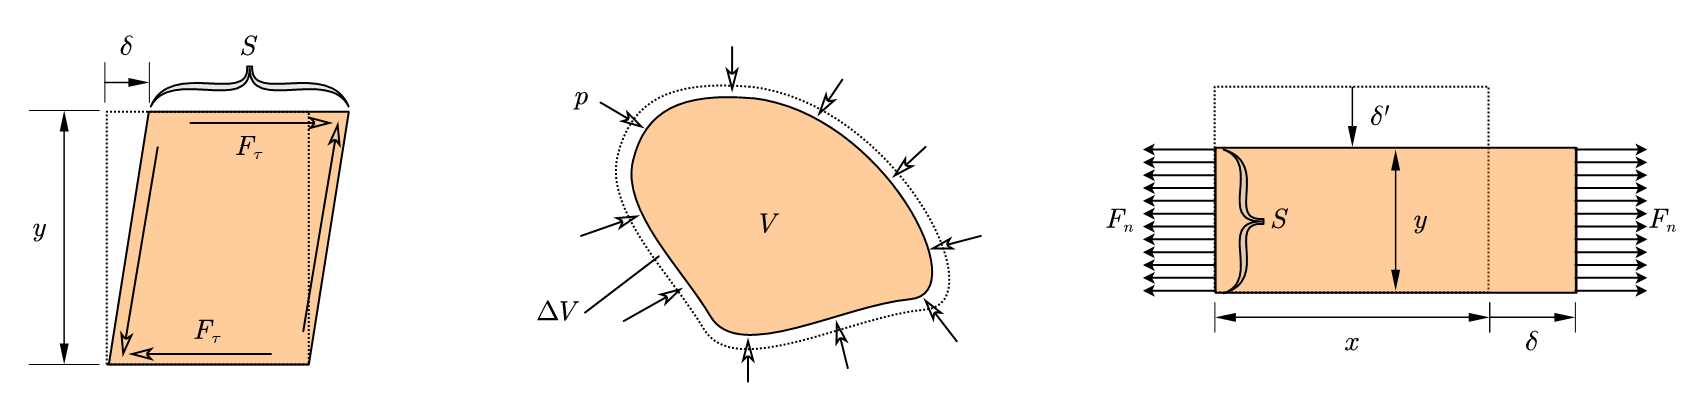
\includegraphics[width=14cm]{image/6-7-3.png}
\caption{剪变模量,\,体弹性模量与杨氏模量}
\end{figure}

三个弹性模量的单位也是应力的单位,\,即帕斯卡,\,而典型材料的弹性模量在$10^{10}{\rm Pa}$的数量级.


\section{弹性棒,\,弹性绳,\,弹性膜与弹性体}

\section{弹性波}

